\subsubsubsubsection{Crossing}
\begin{figure}[h]
\centering
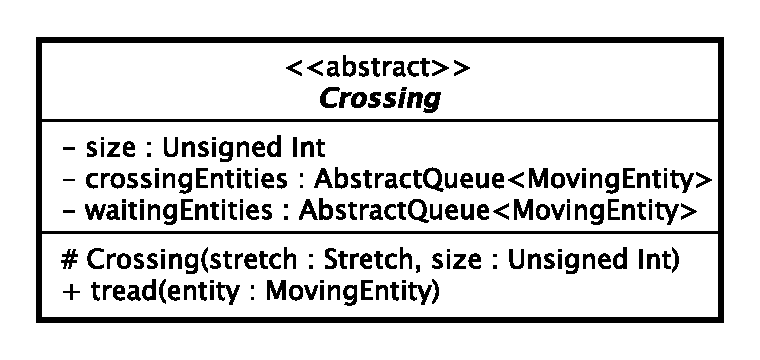
\includegraphics[scale=0.6,keepaspectratio]{images/solution/crossing.eps}
\caption{App::Reactive::Crossing}
\label{fig:sd-app-crossing}
\end{figure}
\FloatBarrier
\begin{itemize}
  \item \textbf{Description} \\
    It represents the zebra crossing entity. 
  \item \textbf{Attribute}
  \begin{itemize}
    \item \texttt{- size: Unsigned Int} \\
The size of the stretch/zcrossing queue.
    \item \texttt{- zcrossing: AbstratQueue<MovingEntity>} \\
The queue of entities which are granted to cross the zebra crossing stretch.
  \item \texttt{- zwaiting: AbstratQueue<MovingEntity>} \\
The queue of entities which are currently waiting to cross the zebra crossing stretch.
  \end{itemize}
\item \textbf{Operation}
  \begin{itemize}
    \item \texttt{+ Crossing(component: Stretch, size: Unsigned Int)} \\
Creates a crossing with a specific component and two queues, the zcrossing queue
has a fixed size.
    \item \texttt{+ tread(entity: MovingEntity)} \\
Implements the treading of the stretch. This decoration allows all the zcrossing entities 
to tread the crossing before each entity in the treading queue. 
  \end{itemize}
\end{itemize}
